\documentclass[11pt,letterpaper]{article}
\usepackage{naaclhlt2010}
\usepackage{times}
\usepackage{latexsym}
\usepackage{hyperref}
\usepackage{graphicx}
\usepackage{wrapfig}
\usepackage{url}
\usepackage{wrapfig}
\usepackage{color}
\usepackage{marvosym}
\usepackage{enumerate}
\usepackage{tikz}
\usepackage{amsmath}
\usepackage{amssymb}
\usepackage{hyperref}
\usepackage{bbm}
\usepackage[T1]{fontenc}
\usepackage{xcolor}
\usepackage{tabu}
\usepackage{colortbl}
\usepackage{subfigure}

\DeclareMathOperator*{\argmax}{arg\,max}

\setlength\titlebox{4cm}    % Expanding the titlebox


\newcommand{\vwi}{{\bf w}_i}
\newcommand{\vw}{{\bf w}}
\newcommand{\vx}{{\bf x}}
\newcommand{\vy}{{\bf y}}
\newcommand{\vb}{{\bf b}}
\newcommand{\valpha}{{\bf \alpha}}
\newcommand{\vxi}{{\bf x}_i}
\newcommand{\yi}{y_i}
\newcommand{\vxj}{{\bf x}_j}
\newcommand{\vxn}{{\bf x}_n}
\newcommand{\yj}{y_j}
\newcommand{\ai}{\alpha_i}
\newcommand{\aj}{\alpha_j}
\newcommand{\X}{{\bf X}}
\newcommand{\Y}{{\bf Y}}
\newcommand{\vz}{{\bf z}}
\newcommand{\msigma}{{\bf \Sigma}}
\newcommand{\vmu}{{\bf \mu}}
\newcommand{\vmuk}{{\bf \mu}_k}
\newcommand{\msigmak}{{\bf \Sigma}_k}
\newcommand{\vmuj}{{\bf \mu}_j}
\newcommand{\msigmaj}{{\bf \Sigma}_j}
\newcommand{\pij}{\pi_j}
\newcommand{\pik}{\pi_k}
\newcommand{\D}{\mathcal{D}}
\newcommand{\el}{\mathcal{L}}
\newcommand{\N}{\mathcal{N}}
\newcommand{\vxij}{{\bf x}_{ij}}
\newcommand{\vt}{{\bf t}}
\newcommand{\yh}{\hat{y}}
\newcommand{\code}[1]{{\footnotesize \tt #1}}
\newcommand{\alphai}{\alpha_i}

\title{2D Visualizations for Support Vector Machine and Neural Network}

\author{Jizhou Xu \, Aileme Omogbai \\
	Johns Hopkins University \\
	{\tt $\{jxu55, aomogba1\}$@jhu.edu}}

\date{December 10, 2014}

\begin{document}
\maketitle
\begin{abstract}
We present a web-based demo that helps to visualize the operations and results of some machine learning binary classification algorithms. For this project, we have chosen to implement two non-linear methods, namely Support Vector Machines (SVM) and Artificial Neural Networks. This visualization tool is implemented fully in Javascript and so the data collection,  training  and display of the results is done on the client-side. It displays a 2D canvas such that data points can be added with mouse clicks and the decision boundary generated by the algorithm is displayed. The data points correspond to the $(x,y)$ positions of the points clicked on the canvas. There is also provision for adjusting some parameters of the model. The visualization can be found at \url{http://metoerite-j.github.io/Visual-Machine-Learning}.
\end{abstract}

\section{Introduction}

In the field of machine learning, binary classification problems stem from the need to separate a set of data points into two different classes. In the supervised case, we have data that is already separated such that each data point belongs to one of the defined classes. For the unsupervised case, we do not know the classes for the example data available. In both cases, we wish to find a model that can learn parameters for the classification such that new unlabeled data points can be assigned to the right class. The model therefore creates "boundaries" such that a data point is labeled according to the side of the boundary that it falls in. 

If the boundary used to separate the two sets of data points is a line, then the problem is a linear classification problem. The data is not usually linearly separable and so complex functions may be needed to define the boundary. Also, while it is intuitive to visualize the concept of the boundary in 2 dimensions, the data is usually of much higher dimensions. This means that very complex decision boundaries are needed to bring about separation in practical applications. Even in 2D, it may be difficult to picture the boundary that is generated by non-linear classifiers, and that is what this project aims to help with.

We present a web visualization tool that shows the classification results of two popular non-linear classifiers. The user is presented with a 2D canvas that contains default points that have been generated with a normal distribution and classified randomly. The classes used for the demo are represented by the colors black/white and this used to label the data points and the regions on the canvas. So, a point is labeled either black or white. Also, the color of any position in the canvas represents the class that a test data point (i.e. a point we want to classify) will be assigned to by the current model. Therefore, the boundary between the white and black regions on the canvas represent the decision boundary that was generated by the algorithm used. 

At the current stage, we have implemented two popular non-linear classifiers: Support Vector Machines (SVM) and Artificial Neural Network (ANN). For training the SVM, we used the Primal Estimated Sub-Gradient Solver for SVM (Pegasos) algorithm. For neural networks training, we used the feed-forward back-propagation neural network as our model. 
SVMs are effective and popular classification learning tool. 

\begin{figure*}
\centering
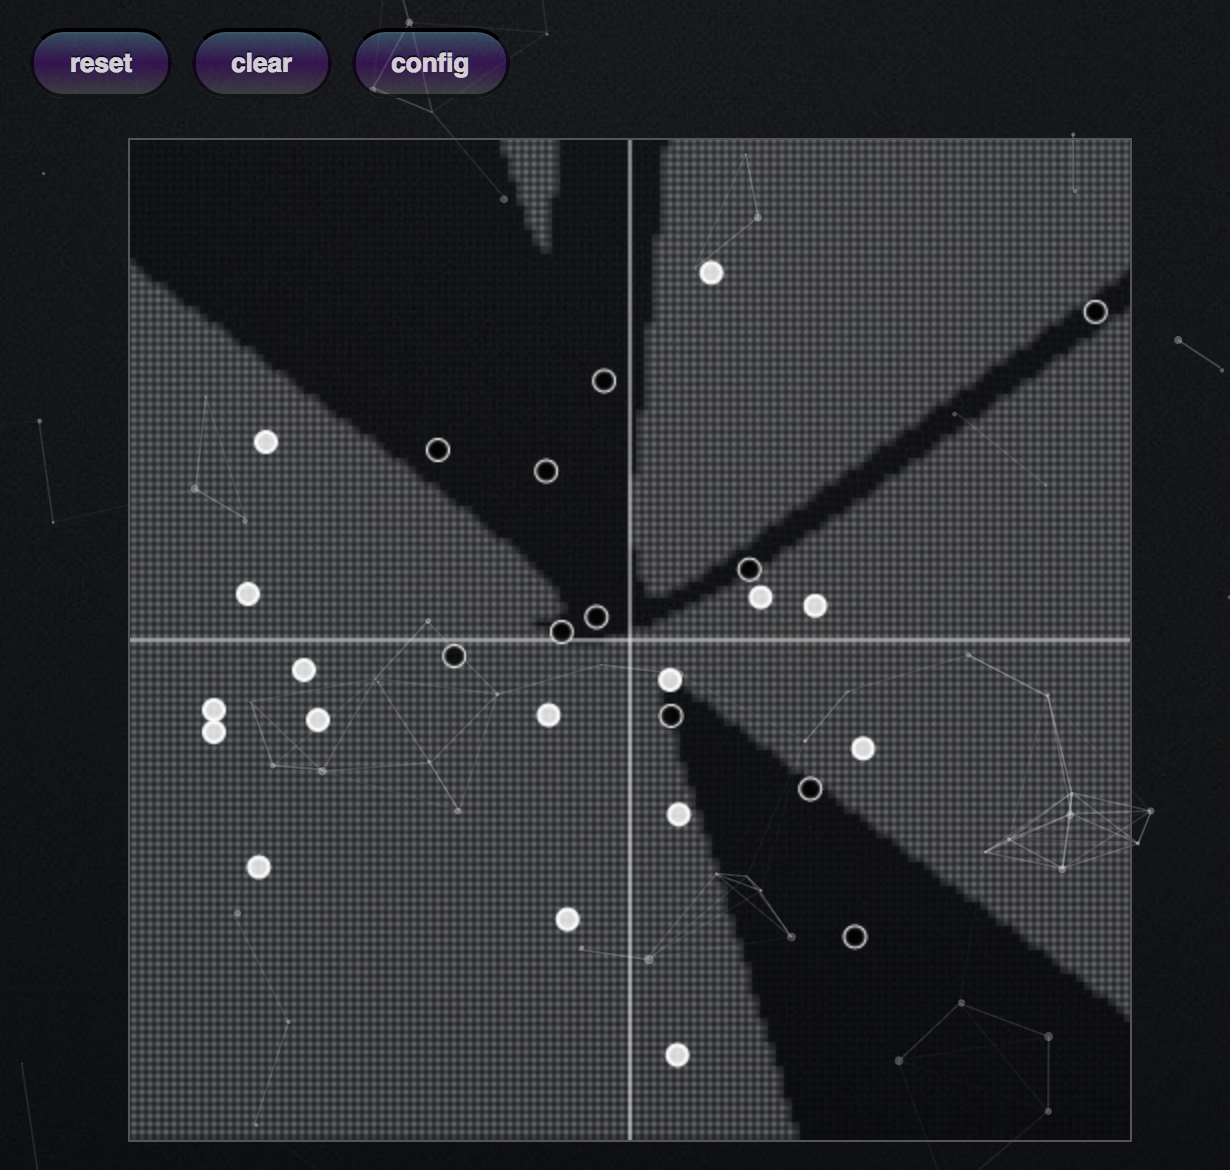
\includegraphics[scale=.5]{images/Intro.PNG}
\caption{Sample output}
\label{fig:intro}
\end{figure*}

\section{SVM}

\subsection{Background}
	The SVM is a very popular model for classification. In the SVM model, data points are seen as points in the $m$-dimensional plane defined by the data. The intuition is that we want to separate the data points with an $(m-1)$-dimensional hyperplane which corresponds to a linear separation. We want to choose the separating line such that its distance to the nearest data point on each side is maximized, which is called maximizing the margin. So we learn the weights in each dimension for that hyperplane. The data points that are closest to the separating hyperplane, that is the data points that affect the position of the hyperplane are called the support vectors. Formally, given a training set $\{(\vxi,\yi)\}_{i=1}^N$, where $\vx_i \in \mathbb{R}^M$ and $y_i \in\{+1,-1\}$, we want to solve the constrained the problem:
\begin{align}
\argmax_{\valpha >= 0} \min_{\vw,b} \{ \frac{1}{2} ||w||^2  - \sum_i^N \alpha_i\left[\yi(\vw \vx - b) - 1\right]  \}
\end{align}
where $b$ is the bias term that determines the offset of the hyperplane from the origin, $w$ denotes the normal vector to the hyperplane and $\alpha$ are Lagrange multipliers. This equation is known as the primal formulation of the optimization problem.

What makes SVMs very popular is that they can be made into non-linear classifiers by applying the "kernel trick". The algorithm is essentially the same except that the dot product used to compute the margins is replaced with a kernel function that represents a dot product also, but in a higher dimension. In this project, we used the radial basis function (RBF) kernel to separate non-linearly separable data.

\begin{figure}
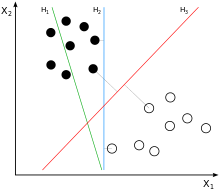
\includegraphics[scale=1]{images/Svm_separating_hyperplanes.PNG}
\caption{SVM margins [Wikipedia]}
\end{figure}

\subsection{Training}
There are different algorithms for training SVMs like:
\begin{enumerate}
\item
the Sequential Minimal Optimization (SMO) \cite{Platt}, and
\item
Primal Estimated sub-GrAdient SOlver for SVM (Pegasos).
\end{enumerate} 

We chose to implement the Pegasos algorithm for training the SVM in this project. The basic algorithm involves using stochastic gradient descent to solve the primal formulation of the problem in $w$ which corresponds to the linear SVM. However, as explained  in the Pegasos formulation\cite{Shalev-Shwartz}, the algorithm can also be modified to handle the non-linear kernelized case as well. We have implemented both versions of the algorithm, so the user can try both the linear and kernel forms to see the boundaries generated by each model type. The application also makes it possible for the user to generate synthetic linearly separable data in order to see the linear SVM solution better. 

\subsection{Implementation}
The implementation of the SVM visualization is divided into two sections. This applies to the other models as well. The actual implementation of the Pegasos algorithm is in a Javascript file(Pegasos.js) that is separate from the actual visualization page. That file contains the code for training the SVM, predicting the class of points after training and all other functions necessary for the training algorithm to work. The usage is as follows:
\begin{enumerate}[i]
\item
Create a new instance of the Pegasos trainer: $pegasos.SVM$.
\item
Call the $train$ method, passing in the data points, the labels and the options for training. Some of the options include: the value of $\lambda$ used in the Pegasos algorithm, number of iterations to be run, the type of kernel ("linear" for linear SVM, and for now "rbf" for RBF kernel), and the value of $\sigma$ for the RBF kernel.
\item
After training, call $predictOne$ to predict a specific data point, or $predict$ for a set of points.
\end{enumerate}
The linear and kernelized versions of the Pegasos are quite different and so they are implemented separately and used depending on which is specified in the training options. For the linear case, the model parameters are the $w$ values but in the kernelized version, its easier to keep the parameters as $\alpha$, the Lagrangian multipliers. These values are used to predict the class of points after training.

The visualization page calls the training algorithm and displays the results on the canvas. Once the page is loaded, default data points corresponding to points on the canvas are generated from a Gaussian distribution and classified arbitrarily. The data is used to train the model. For drawing the data points, boundaries and many finicky details of 2D drawing with Javascript, we made use of a library written by Andrej Karpathy \cite{Andrej}. To display the decision boundary, we predict the class of every point on the canvas. The boundary is seen as the separation between the white and dark regions on the canvas.

The user is able to switch from a linear SVM to using a kernel and the model is retrained appropriately and the decision boundary displayed. For the linear SVM, we show the decision boundary and the margins of the classifier. Because the default data generated is not likely to be linearly separable, we provided an option to clear the points and input new data points. This can be used to generate linearly separable data, because the linear classifier will not produce sensible boundaries for non-linear data.

It is also possible to vary the value of the parameter of the RBF kernel $\sigma$, which has a big effect on the shape of the decision boundary. By the definition of the kernel, small values of $\sigma$ will make it such that only points close to each other will affect prediction because the value of the kernel will be close to zero for points far from each other. The model will look to be overfitting the data. For large values of $\sigma$, we get smooth boundaries that mis-classifies points, tending towards a linear classifier.

\subsection{Results}
See Figure \ref{fig:svm}
\begin{figure}
\hfill
\subfigure[Linear]{\includegraphics[scale=.2]{images/PEGASOS-Linear.png}}
\hfill
\subfigure[RBF: $\sigma=1$]{\includegraphics[scale = .2]{images/PEGASOS-1.png}}
\hfill
\caption{SVM decision boundaries}
\end{figure}
\begin{figure}
\subfigure[RBF: $\sigma=3.2$]{\includegraphics[scale = .2]{images/PEGASOS-32.png}}
\hfill
\subfigure[RBF: $\sigma=3.2$]{\includegraphics[scale = .2]{images/PEGASOS-32.png}}
\hfill
\caption{SVM decision boundaries}
\label{fig:svm}
\end{figure}

\section{ANN}

\subsection{Background}

In machine learning, ANNs are a family of statistical learning algorithms and are used to estimate or approximate functions. An Artificial Neural Network (ANN) can be regarded as an information processing paradigm that is inspired by the way biological nervous systems, such as the brain, process information.  The key element of this paradigm is the novel structure of the system. It is composed of a large number of highly interconnected nodes ("neurons") in different layers working together to produce a final output.  This field was established before the advent of computers, and has survived at least one major setback and several eras.

We used one of the easiest neural networks - the feedforward neural network. The key distinction here is that information moves only in one direction in the network. We have a layer of "input" units which is connected to a hierarchy of layers of "hidden" units, the last of which is connected to a layer of "output" units. The network approximates a function by assigning weights to each node for the data it receives from the nodes in the layer before it. The sum of the products of the weights and inputs is taken for each node and if the value is up to a certain threshold, the node is activated. The function that implements this is called the activation function. We use a sigmoid function to achieve that here. This is also used at the final layer to decide the class for the input data in our classification problem.

\subsection{Training}
We used the back propagation algorithm to train the neural network model. This involves getting the error in the output i.e. the difference between the output and the target output and propagating it backwards through the layers. The errors are then used to adjust the weights of the nodes such that the loss function is minimized usually using gradient descent. The update equation takes a simple form because the activation function is the sigmoid function. This process is repeated for all the input data and for many iterations until convergence.

\subsection{Implementation}
The structure of our implementation is similar to the SVM implementation described earlier. The data and options for the training schedule is passed into the neural net implementation code. Some of the options are the learning rate and the configuration of the network in terms of the number of hidden layers and the number of nodes in each layer.  The procedure is different here because the training method is called for many iterations until the mode converges. Here we say it has converged when the mean squared error (MSE) on the training set reaches a certain minimum. This ensures that the model does not run forever on the client system. 

Prediction is basically forward propagation on the input point and we predict 1(black) if the output $>$ 0.5, and 0(white) otherwise.

The user is able to experiment with the network configuration to see how it affects the boundary. It should be noted that the objective function is non-convex and so the model may converge to an obviously wrong solution. In such cases, it may be necessary to adjust the weights so that another solution is gotten but we have not implemented that here.

\subsection{Results}
See Figure \ref{fig:nn}
\begin{figure}
\hfill
\subfigure[2 hidden layers, 10 nodes each]{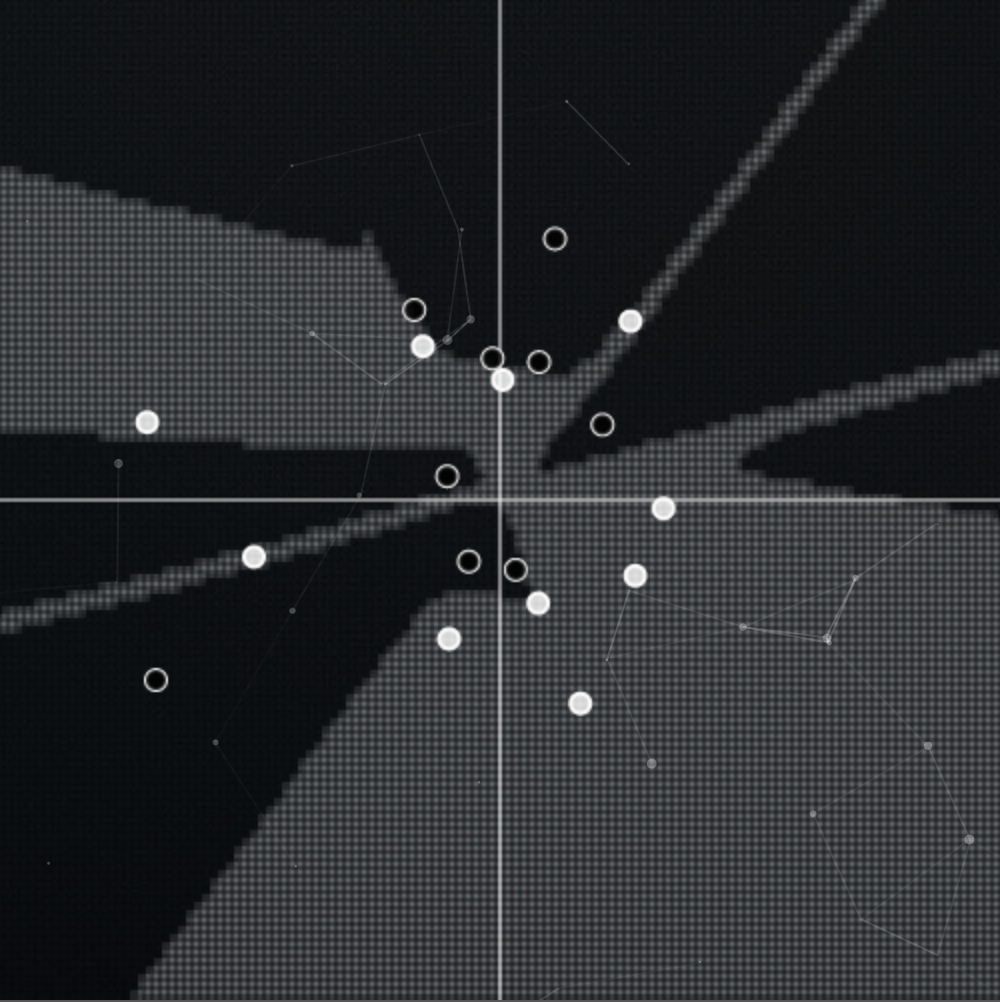
\includegraphics[scale=.2]{images/2-10-10-1.png}}
\hfill
\subfigure[3 hidden layers, 15 nodes each]{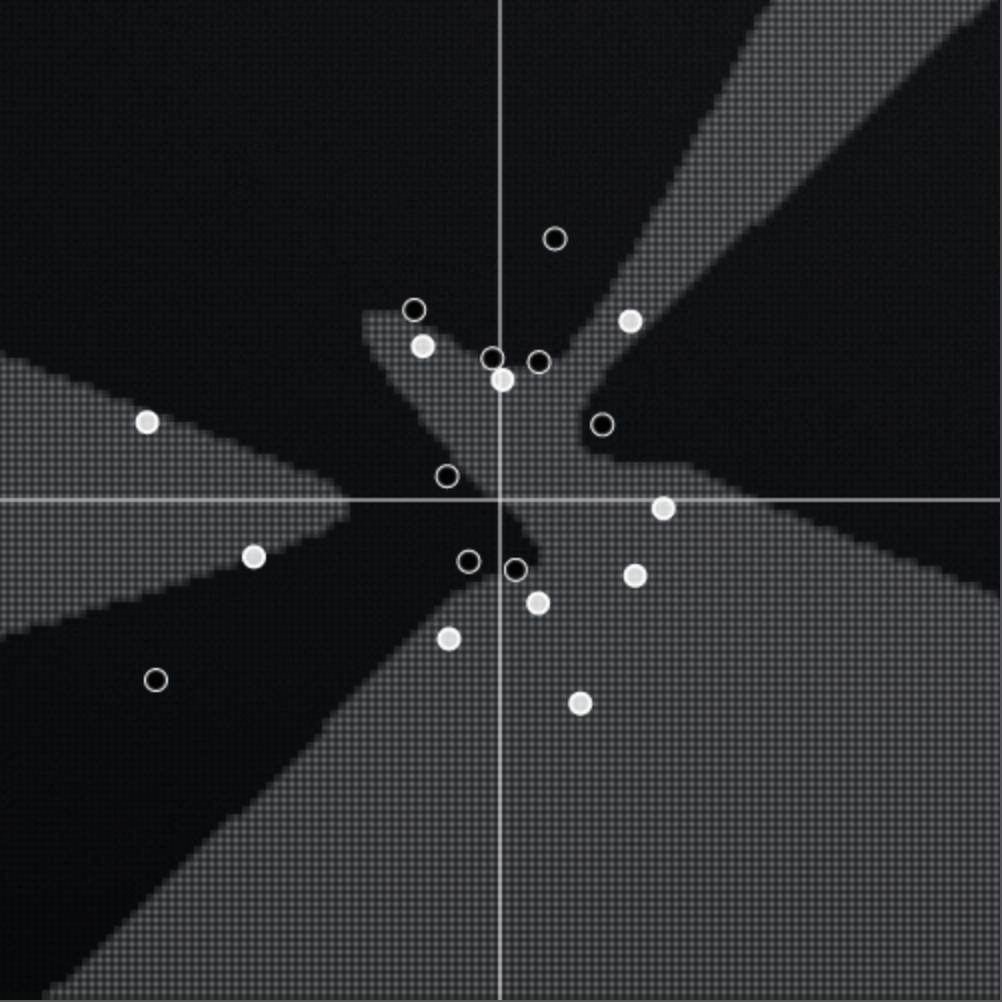
\includegraphics[scale=.2]{images/2-15-10-5-1.png}}
\hfill
\caption{Neural Network decision boundaries}
\label{fig: nn}
\end{figure}


\section{Comparison To Proposal}

\taburowcolors[2]{white .. black!20}

\sffamily\footnotesize
\tabulinesep=6pt
\begin{tabu}{|>{\cellcolor{black!60}\color{white}}r|X[cm]|X[cm]|}
\hline
\rowcolor{black!80}\strut  Factors & \color{white}Plan & \color{white}Actual Achievment \\
UI & clean & somewhat cool \\
number of algorithms & 2 & 2 \\
parameters & adjustable & some are adjustable \\
speed & no crash & fast enough except for ANN\\
tutorial & readable & detailed \\
\hline
\end{tabu}


We successfully implemented both of our target algorithms. In our proposal, we mentioned we would like to do a comparative analysis for similar algorithms. However, we couldn't 

The two SVMs we presented handle both linear and non-linear datasets. We used the RBF kernel, and we didn't have enough time to add more options, but the RBF $\sigma$ is adjustable.

For the ANN, the number of layers and the number of neurons in each layer are both adjustable, and the configuration is displayed whenever a change is made.

\section{Extensions}
The machine learning algorithms implemented here are supervised learning algorithms. The demo can be extended to include more complex learning methods as well. K-means for example, is an algorithm that may be useful to visualize. Deep networks particularly has attracted a lot of attention in recent times and a good number of online demos can actually be found on GitHub currently.

\begin{thebibliography}{}

\bibitem[\protect\citename{Platt} 1998]{Platt:72}
{John C. Platt}.
\newblock {\em Fast Training of Support Vector Machines using Sequential Minimal Optimization}.
\newblock MIT Press, Cambridge, MA.

\bibitem[\protect\citename{Shalev-Shwartz} 2007]{}
{Shai Shalev-Shwartz, Yoram Singer, Nathan
Srebro, Andrew Cotter}.
\newblock {\em Pegasos: Primal Estimated sub-GrAdient SOlver for SVM}.

\bibitem[\protect\citename{Andrej}]{}
{Andrej Karpathy}.
\newblock {\em notpygamejs: \url{https://github.com/karpathy/notpygamejs}}.

\bibitem[\protect\citename{Andrej Karpathy}]{}
{Andrej Karpathy}.
\newblock {\em Machine Learning demos in Javascript: \url{http://cs.stanford.edu/people/karpathy/svmjs/demo/}}.

\end{thebibliography}

\end{document}
